\chapter*{Annexe A : Diagrammes UML du Projet CIRCULI}
\addcontentsline{toc}{chapter}{Annexe A : Diagrammes UML}

\section{Diagramme de Cas d'Utilisation}

\begin{figure}[H]
    \centering
    \begin{tikzpicture}[
        actor/.style={circle, draw, minimum size=1.5cm, thick},
        usecase/.style={ellipse, draw, minimum width=2.5cm, minimum height=1cm, thick},
        association/.style={thick},
        include/.style={->, thick, dashed},
        scale=1.1
    ]
    
    % Acteurs
    \node[actor] (agent) at (0, 5) {Agent Municipal};
    \node[actor] (citoyen) at (0, 2) {Citoyen};
    \node[actor] (admin) at (0, -1) {Administrateur};
    
    % Système CIRCULI
    \draw[thick, rounded corners=0.5cm] (3, -2) rectangle (9, 6.5);
    \node at (9.2, 6.2) {\textbf{CIRCULI}};
    
    % Cas d'utilisation
    \node[usecase] (visualiser) at (6, 5.5) {Visualiser trafic\\en temps réel};
    \node[usecase] (generer) at (6, 3.8) {Générer rapport\\hebdomadaire};
    \node[usecase] (consulter) at (6, 2.2) {Consulter indicateurs\\KPI};
    \node[usecase] (telecharger) at (6, 0.8) {Télécharger données};
    \node[usecase] (configurer) at (6, -0.8) {Configurer caméras\\et ROI};
    \node[usecase] (gerer) at (6, -1.8) {Gérer utilisateurs\\et accès};
    
    % Associations acteur-cas
    \draw[association] (agent) -- (visualiser);
    \draw[association] (agent) -- (generer);
    \draw[association] (agent) -- (consulter);
    \draw[association] (citoyen) -- (consulter);
    \draw[association] (citoyen) -- (telecharger);
    \draw[association] (admin) -- (configurer);
    \draw[association] (admin) -- (gerer);
    
    \end{tikzpicture}
    \caption{Diagramme de cas d'utilisation – Interactions utilisateurs avec CIRCULI}
    \label{fig:use-case}
\end{figure}

\newpage
\section{Diagramme de Classe}

\begin{figure}[H]
    \centering
    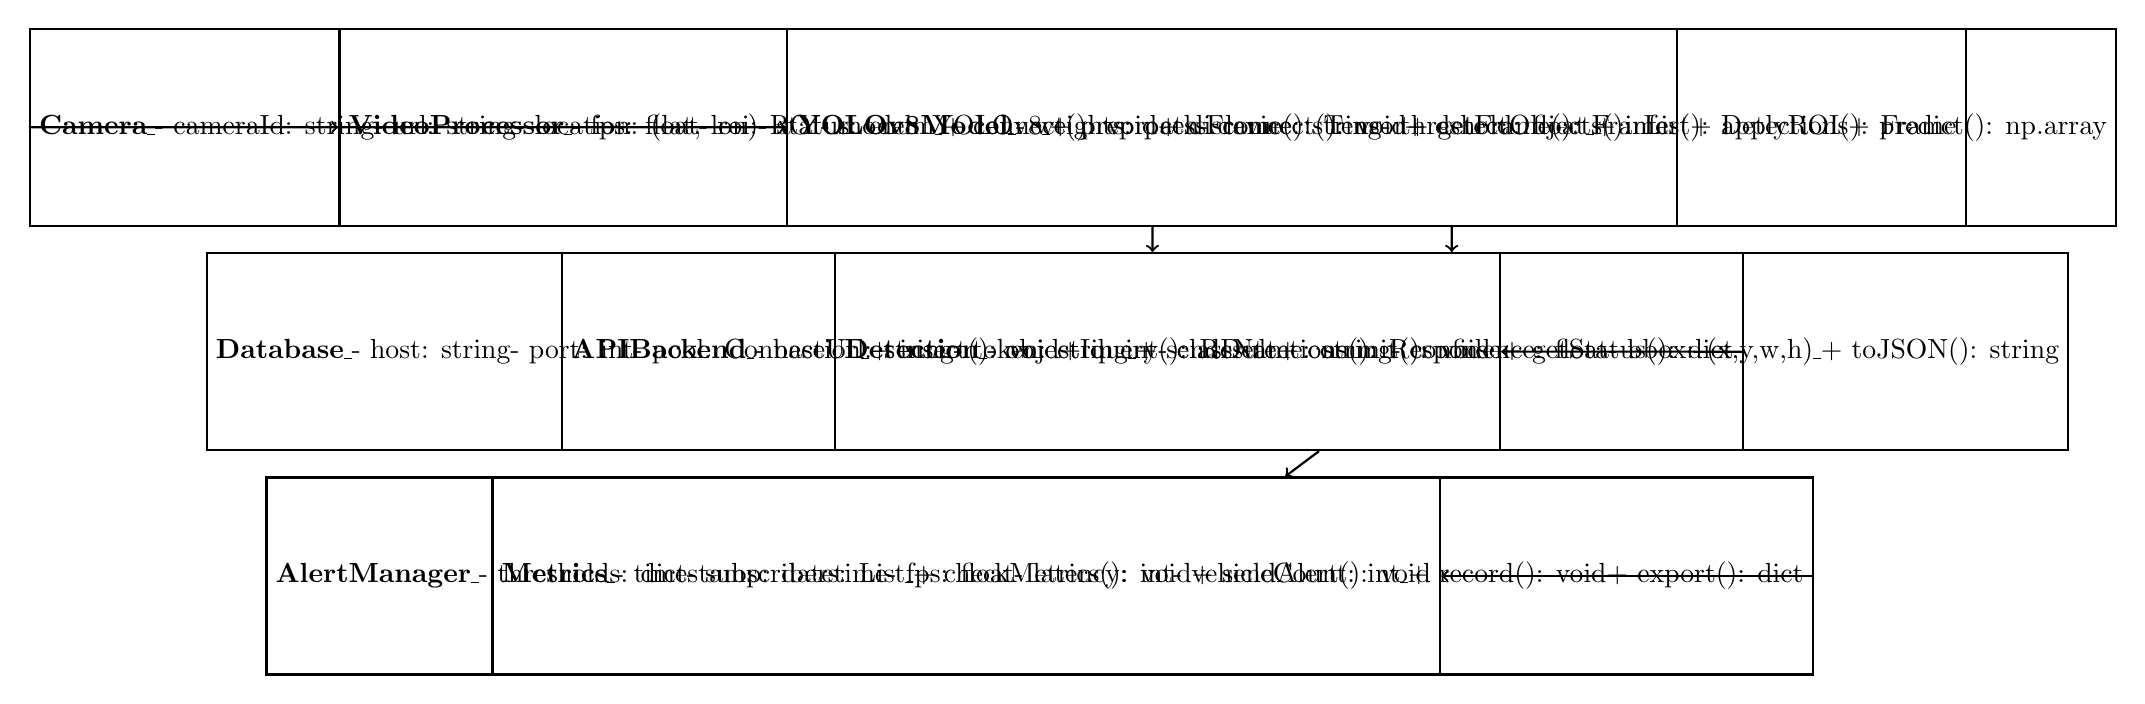
\begin{tikzpicture}[
        class/.style={rectangle, draw, minimum width=3cm, minimum height=2.5cm, thick},
        scale=0.95
    ]
    
    % Classe Camera
    \node[class] (camera) at (1, 8) {
        \textbf{Camera}\\
        \line(1,0){2.8}\\
        - cameraId: string\\
        - url: string\\
        - location: (lat, lon)\\
        - status: enum\\
        \line(1,0){2.8}\\
        + connect(): void\\
        + disconnect(): void\\
        + getFrame(): Frame
    };
    
    % Classe VideoProcessor
    \node[class] (processor) at (5, 8) {
        \textbf{VideoProcessor}\\
        \line(1,0){2.8}\\
        - fps: float\\
        - roi: ROI\\
        - model: YOLOv8\\
        \line(1,0){2.8}\\
        + preprocessFrame(): Tensor\\
        + detectObjects(): List\\
        + applyROI(): Frame
    };
    
    % Classe YOLOv8Model
    \node[class] (yolo) at (9, 8) {
        \textbf{YOLOv8Model}\\
        \line(1,0){2.8}\\
        - weights: path\\
        - device: string\\
        - threshold: float\\
        \line(1,0){2.8}\\
        + infer(): Detections\\
        + predict(): np.array
    };
    
    % Classe Detection
    \node[class] (detection) at (9, 5) {
        \textbf{Detection}\\
        \line(1,0){2.8}\\
        - objectId: int\\
        - className: string\\
        - confidence: float\\
        - bbox: (x,y,w,h)\\
        \line(1,0){2.8}\\
        + toJSON(): string
    };
    
    % Classe APIBackend
    \node[class] (api) at (5, 5) {
        \textbf{APIBackend}\\
        \line(1,0){2.8}\\
        - baseUrl: string\\
        - token: string\\
        \line(1,0){2.8}\\
        + sendDetections(): Response\\
        + getStatus(): dict
    };
    
    % Classe Database
    \node[class] (db) at (1, 5) {
        \textbf{Database}\\
        \line(1,0){2.8}\\
        - host: string\\
        - port: int\\
        - pool: Connection\\
        \line(1,0){2.8}\\
        + insert(): void\\
        + query(): Result\\
        + commit(): void
    };
    
    % Classe Metrics
    \node[class] (metrics) at (5, 2) {
        \textbf{Metrics}\\
        \line(1,0){2.8}\\
        - timestamp: datetime\\
        - fps: float\\
        - latency: int\\
        - vehicleCount: int\\
        \line(1,0){2.8}\\
        + record(): void\\
        + export(): dict
    };
    
    % Classe AlertManager
    \node[class] (alert) at (1, 2) {
        \textbf{AlertManager}\\
        \line(1,0){2.8}\\
        - thresholds: dict\\
        - subscribers: List\\
        \line(1,0){2.8}\\
        + checkMetrics(): void\\
        + sendAlert(): void
    };
    
    % Associations
    \draw[thick, ->] (camera) -- (processor);
    \draw[thick, ->] (processor) -- (yolo);
    \draw[thick, ->] (yolo) -- (detection);
    \draw[thick, ->] (processor) -- (api);
    \draw[thick, ->] (api) -- (db);
    \draw[thick, ->] (detection) -- (metrics);
    \draw[thick, ->] (metrics) -- (alert);
    
    \end{tikzpicture}
    \caption{Diagramme de classe – Architecture logicielle de CIRCULI}
    \label{fig:class-diag}
\end{figure}

\newpage
\section{Diagramme de Séquence – Scénario Principal}

\subsection{Flux global de traitement (de la caméra à la visualisation)}

\begin{figure}[H]
    \centering
    \begin{tikzpicture}[
        scale=1,
        actor/.style={rectangle, draw, minimum width=1.8cm, minimum height=0.6cm},
        object/.style={rectangle, draw, minimum width=1.8cm, minimum height=0.6cm},
        message/.style={->, thick, black}
    ]
    
    % Acteurs / Objets
    \node[actor] (camera) at (0, 10) {Camera RTSP};
    \node[object] (processor) at (2.5, 10) {VideoProcessor};
    \node[object] (yolo) at (5, 10) {YOLOv8};
    \node[object] (api) at (7.5, 10) {APIBackend};
    \node[object] (db) at (10, 10) {Database};
    
    % Lignes de vie
    \draw[dashed] (camera) -- (camera |- -0.5);
    \draw[dashed] (processor) -- (processor |- -0.5);
    \draw[dashed] (yolo) -- (yolo |- -0.5);
    \draw[dashed] (api) -- (api |- -0.5);
    \draw[dashed] (db) -- (db |- -0.5);
    
    % Messages
    \draw[message] (camera) -- (processor) node[midway, above, font=\small] {1: readFrame()};
    \draw[message] (processor) -- (processor |- 8.5) node[midway, right, font=\small] {2: applyROI()};
    \draw[message] (processor) -- (processor |- 7.8) node[midway, right, font=\small] {3: normalize()};
    \draw[message] (processor) -- (yolo) node[midway, above, font=\small] {4: infer(tensor)};
    \draw[message] (yolo) -- (processor) node[midway, above, font=\small] {5: detections[]};
    \draw[message] (processor) -- (api) node[midway, above, font=\small] {6: sendDetections(list)};
    \draw[message] (api) -- (db) node[midway, above, font=\small] {7: insert(records)};
    \draw[message] (db) -- (api) node[midway, above, font=\small] {8: ACK};
    \draw[message] (api) -- (processor) node[midway, above, font=\small] {9: success};
    
    \end{tikzpicture}
    \caption{Diagramme de séquence – Flux de traitement d'une frame vidéo}
    \label{fig:seq-main}
\end{figure}

\subsection{Sous-diagramme 1 : Inférence YOLOv8}

\begin{figure}[H]
    \centering
    \begin{tikzpicture}[
        scale=1,
        object/.style={rectangle, draw, minimum width=1.8cm, minimum height=0.6cm},
        message/.style={->, thick, black}
    ]
    
    \node[object] (tensor_prep) at (0, 10) {Tensor};
    \node[object] (model) at (2.5, 10) {YOLOv8Model};
    \node[object] (nms) at (5, 10) {NMS Filter};
    \node[object] (results) at (7.5, 10) {Detections};
    
    \draw[dashed] (tensor_prep) -- (tensor_prep |- -0.5);
    \draw[dashed] (model) -- (model |- -0.5);
    \draw[dashed] (nms) -- (nms |- -0.5);
    \draw[dashed] (results) -- (results |- -0.5);
    
    \draw[message] (tensor_prep) -- (model) node[midway, above, font=\small] {1: forward(x)};
    \draw[message] (model) -- (model |- 8.5) node[midway, right, font=\small] {2: grid\_predictions};
    \draw[message] (model) -- (nms) node[midway, above, font=\small] {3: raw\_boxes};
    \draw[message] (nms) -- (nms |- 7.2) node[midway, right, font=\small] {4: filter(iou<0.4)};
    \draw[message] (nms) -- (results) node[midway, above, font=\small] {5: filtered\_list};
    
    \node at (3.75, -1.5) {\small \textit{Détail : passage de la prédiction brute au filtrage NMS (confiance + IoU)}};
    
    \end{tikzpicture}
    \caption{Sous-diagramme 1 – Étapes d'inférence du modèle YOLOv8}
    \label{fig:seq-yolo}
\end{figure}

\subsection{Sous-diagramme 2 : Gestion des erreurs et résilience}

\begin{figure}[H]
    \centering
    \begin{tikzpicture}[
        scale=1,
        object/.style={rectangle, draw, minimum width=1.8cm, minimum height=0.6cm},
        message/.style={->, thick, black},
        error/.style={->, thick, red}
    ]
    
    \node[object] (camera) at (0, 10) {Camera};
    \node[object] (processor) at (2.5, 10) {Processor};
    \node[object] (api) at (5, 10) {APIBackend};
    \node[object] (alert) at (7.5, 10) {AlertManager};
    
    \draw[dashed] (camera) -- (camera |- -0.5);
    \draw[dashed] (processor) -- (processor |- -0.5);
    \draw[dashed] (api) -- (api |- -0.5);
    \draw[dashed] (alert) -- (alert |- -0.5);
    
    \draw[message] (camera) -- (processor) node[midway, above, font=\small] {1: readFrame()};
    \draw[error] (processor) -- (processor |- 8.2) node[midway, right, font=\small, color=red] {2: timeout!};
    \draw[error] (processor) -- (alert) node[midway, above, font=\small, color=red] {3: onError(RTSP\_DOWN)};
    \draw[message] (alert) -- (alert |- 7.5) node[midway, right, font=\small] {4: log + notify};
    \draw[message] (processor) -- (processor |- 6.8) node[midway, right, font=\small] {5: retry(backoff=2s)};
    \draw[message] (camera) -- (processor) node[midway, above, font=\small] {6: readFrame() [RETRY]};
    \draw[message] (processor) -- (api) node[midway, above, font=\small] {7: sendDetections()};
    
    \node at (3.75, -1.5) {\small \textit{Gestion : timeout réseau → log → alerte → retry exponentiel}};
    
    \end{tikzpicture}
    \caption{Sous-diagramme 2 – Flux de gestion des erreurs et résilience}
    \label{fig:seq-error}
\end{figure}

\subsection{Sous-diagramme 3 : Cycle de mise à jour des KPI}

\begin{figure}[H]
    \centering
    \begin{tikzpicture}[
        scale=1,
        object/.style={rectangle, draw, minimum width=1.8cm, minimum height=0.6cm},
        message/.style={->, thick, black}
    ]
    
    \node[object] (detections) at (0, 10) {Detections};
    \node[object] (metrics) at (2.5, 10) {Metrics};
    \node[object] (db) at (5, 10) {Database};
    \node[object] (grafana) at (7.5, 10) {Grafana};
    
    \draw[dashed] (detections) -- (detections |- -0.5);
    \draw[dashed] (metrics) -- (metrics |- -0.5);
    \draw[dashed] (db) -- (db |- -0.5);
    \draw[dashed] (grafana) -- (grafana |- -0.5);
    
    \draw[message] (detections) -- (metrics) node[midway, above, font=\small] {1: record(objects=[])};
    \draw[message] (metrics) -- (metrics |- 8.8) node[midway, right, font=\small] {2: compute FPS};
    \draw[message] (metrics) -- (metrics |- 8.2) node[midway, right, font=\small] {3: compute latency};
    \draw[message] (metrics) -- (db) node[midway, above, font=\small] {4: insert\_metrics()};
    \draw[message] (db) -- (db |- 7.5) node[midway, right, font=\small] {5: persist};
    \draw[message] (db) -- (grafana) node[midway, above, font=\small, sloped] {6: query (every 10s)};
    \draw[message] (grafana) -- (grafana |- 6.5) node[midway, right, font=\small] {7: render\_dashboard};
    
    \node at (3.75, -1.5) {\small \textit{Mise à jour continue des KPI : collection → calcul → persistence → visualisation}};
    
    \end{tikzpicture}
    \caption{Sous-diagramme 3 – Cycle de mise à jour des indicateurs KPI}
    \label{fig:seq-kpi}
\end{figure}

\newpage
\section{Résumé des interactions}

Le tableau suivant synthétise les principaux appels entre composants :

\begin{table}[H]
    \centering
    \resizebox{\textwidth}{!}{
    \begin{tabular}{llll}
        \toprule
        \textbf{Composant Source} & \textbf{Composant Cible} & \textbf{Opération} & \textbf{Fréquence} \\
        \midrule
        Camera & VideoProcessor & readFrame() & Continu (25-30 FPS) \\
        VideoProcessor & YOLOv8 & infer(tensor) & Continu (9-19 FPS après ROI) \\
        YOLOv8 & NMS Filter & filter() & Continu \\
        VideoProcessor & APIBackend & sendDetections() & Chaque détection \\
        APIBackend & Database & insert() & Batch (1x/min) \\
        Metrics & Database & insert\_metrics() & Chaque minute \\
        Database & Grafana & query() & Polling (10s) \\
        AlertManager & Logger & log() & Sur événement \\
        \bottomrule
    \end{tabular}
    }
    \caption{Tableau d'interactions entre composants}
    \label{tbl:interactions}
\end{table}

